% brainstorm:

% * citar fundamento em teorias de contornos e pouco uso em composição
% * exemplos das necessidades de operações na composição (peça do mestrado)
% * desenvolvimento do goiaba (para que serve, exemplo de código e de
% saída)
% * trabalhos futuros

\section{Introduction}
\label{sec:introduction}

Contours can be understood as the shape or format of an object. In
Music, they can be associated to elements like pitch, density, rhythm,
and represent a parameter in function of another, as pitch in function
of time. Contours can be easily recognized from graphic representation
by professionals and laymen alike \cite{marvin88:generalized}. For
instance, Beethoven's Fifth Symphony main motive and its pitch contour
are represented respectively in figures \ref{fig:5a-sinfonia-motivo}
and \ref{fig:c-3120}.

\begin{figure}
  \centering
  \subfloat[Main motive]{
    \includegraphics[scale=.9]{5a-sinfonia}
    \label{fig:5a-sinfonia-motivo}
  }

  \subfloat[Contour (3 1 2 0)]{
    \includegraphics{c-3120}
    \label{fig:c-3120}
  }
  \caption{Fifth Symphony main motive contour}
  \label{fig:5a-sinfonia}
\end{figure}

Contour is defined as an ordered set of distinct elements numbered
from the lowest to the highest \cite{morris93:directions}. In
contours, absolute values of its elements are ignored, and only the
high-low relationship between these elements is regarded. For
instance, figures \ref{fig:5a-sinfonia-motivo} and \ref{fig:ly-3120}
have the same pitch contour, graphically represented in figure
\ref{fig:c-3120}, and symbolically by (3 1 2 0).

The study of Contour is important because, like motives and pitch
sets, contours can help to give coherence to a musical piece. They
represent structural devices that can be combined through operations
like inversion and retrogradation, and can be aproached by analytical
or compositional points of view.

\begin{figure}
  \centering
  \includegraphics{ly-3120-qualquer}
  \caption{A melody with (3 1 2 0) contour}
  \label{fig:ly-3120}
\end{figure}

Contour theories
\cite{friedmann85:methodology,friedmann87:response,morris87:composition,morris93:directions,marvin.ea87:relating,marvin88:generalized,marvin.ea95:generalization,polansky.ea92:possible,quinn97:fuzzy,clifford95:contour,beard03:contour}
have been developed to organize in a systematic way the knowledge
about contour. These theories were developed primarily as analytic
techniques for non-tonal compositions \cite{beard03:contour}, and
provide arrays, matrices and many operations to help the comparison of
contours, like inversion, translation, comparison matrix, and contour
interval array.

Contour operations demand precise mathematical calculations and
graphical representations easy plotting. So a computer program to
process contour can assist composers and analysts in tasks like
operations calculation---avoiding human error and wasting time---,
automated graphical plotting, and conversion from score to contours
and vice-versa. For these reasons we are developing \goiaba{}, a
contour processor software (see section \ref{sec:goiaba}).

\section{Contour applications in composition}
\label{sec:cont-appl-comp}

Systematic studies about the usage of contour operations and
combinations in musical composition are scarce, despite the possible
coherence that contours can give and the operations provided by
contour theories. For this reason we are researching contours usage in
composition. The first author of this paper, in his
master's\footnote{The reference was omitted to keep anonymity. It will
  be included in final version.}, composed a woodwind quintet based on
contour theories operations.

This quintet was composed entirely using \goiaba{} to simplify
operations and plotting. The piece is based on combinations of contour
operations associated to parameters such as pitch, tempo, density and
texture. This quintet is based on P(5 3 4 1 2 0) contour
(fig. \ref{fig:c-534120}, its subsets and operations---retrogradation,
inversion, rotation, interpollation.

\begin{figure}
  \centering
  \includegraphics{c-534120}
  \caption{P(5 3 4 1 2 0) contour}
  \label{fig:c-534120}
\end{figure}

\goiaba{} was essential to compose a \eng{fugato}, in the quintet,
because each piece of subject and countersubject were based on
different combinations of rotation and retrogradation operations.  The
subject has original contour P(5 3 4 1 2 0) and factor 3 rotation
(fig. \ref{fig:sujeito-fugato}). Figure
\ref{fig:output-sujeito-fugato} has the contour software output for
graphical representations of these subject operations. Contoursubject
has original contour retrogradation repeated three times with
different rotation factors---5, 4 and 3
(fig. \ref{fig:contra-sujeito-fugato}). In the same way software
output for these operations are in figure
\ref{fig:output-contra-sujeito-fugato}.

\begin{figure*}
  \centering
  \subfloat[Subject]{
    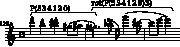
\includegraphics[scale=2.8]{sujeito-fugato}
    \label{fig:sujeito-fugato}
  }

  \subfloat[Countersubject]{
    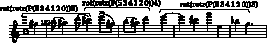
\includegraphics[scale=2.8]{contra-sujeito-fugato}
    \label{fig:contra-sujeito-fugato}
  }
  \caption{Structural elements of \eng{fugato}}
  \label{fig:elementos-fugato}
\end{figure*}

\begin{figure*}
  \centering
  \subfloat[Subject]{
    \includegraphics[scale=.44]{output-subject}
    \label{fig:output-sujeito-fugato}
  }
  \subfloat[Countersubject]{
    \includegraphics[scale=.44]{output-countersubject}
    \label{fig:output-contra-sujeito-fugato}
  }
  \caption{Software output for \eng{fugato} contour operations}
  \label{fig:output-fugato}
\end{figure*}

\section{Goiaba}
\label{sec:goiaba}

\goiaba{}\footnote{Additional information and link were also omitted
  to keep anonymity.} is a software developed in Common Lisp
\cite{graham94:lisp}, compiled with Steel Bank Common Lisp (SBCL)
\cite{team07:sbcl}, and bottom up metodology.

Bottom up methodology is related to the development direction, from
simple subsystems to the entire program. This methodology is suitable
to programs that progressively have complexity increased. Programs
like \TeX{}\footnote{\url{www.tug.org}} and X
Windows\footnote{\url{www.x.org}} are developed in this way. This
metodology has good advantages as the possibility to make smaller and
smarter programs, to reuse subsystems functions in others subsystems,
and to simplify and clear programmer ideas \cite{graham94:lisp}.

In \goiaba{}, contours are symbolic represented in two ways: as simple
contours and duration-included contours. Simple contours represents
only contour element values: \code{(5 9 6)}. Duration-included
contours represents also the time when the element occur: \code{((0
  5)(1 9)(2 6))}. Despite \goiaba{} provides a codification that
includes time influence in contour, we don't consider time. It's a
future work (see section \ref{sec:future-work}).

\goiaba{} has \texttt{ponto}, \texttt{contorno-simples} and
\texttt{contorno-duracao} classes. The \texttt{ponto} class defines
pitches in time as (x, y), cartesian elements, x as time and y as
pitch. The \texttt{contorno-duracao} class defines a contour as a
points list, like ((x, y) (z, w)), and the \texttt{contorno-simples}
class defines contours only as pitches, like (y w).

Some read macros were defined to simplify instances making easier. For
instance, to make \texttt{ponto} instance, it's possible to do
\code{(make-instance 'ponto :x 0 :y 3)} or just \code{\#p(0 3)}, with
read macro. It's possible also to create \texttt{contorno-duracao}
with two points in \code{\#d(\#p(0 3) \#p(1 4))}.

Contour operations are implemented in methods, taking Common Lisp
object systems (CLOS) multiple order. So a method like \texttt{rotate}
behaves in a different way depending on the first parameter. In
following code there are two methods, the first to
\code{contorno-duracao}, and the second to \code{contorno-simples}.

%% FIXME: traduzir termos do goiaba
\begin{figure*}
\begin{verbatim}
(defmethod rotacionar ((objeto contorno-duracao) &optional (fator 1))
  (if (> fator (length (pontos objeto)))
      (let ((x (mapcar #'ponto-x (pontos objeto)))
            (y (mapcar #'ponto-y (pontos objeto))))
        (make-contorno-duracao (mapcar #'make-ponto x
           (append (subseq y fator) (subseq y 0 fator)))))))

(defmethod rotacionar ((objeto contorno-simples) &optional (fator 1))
  (make-contorno-simples (append (subseq (pontos objeto) fator)
                                 (subseq (pontos objeto) 0 fator))))
\end{verbatim}
  \caption{Methods}
  \label{fig:code-methods}
\end{figure*}

%% FIXME: update operations
\goiaba{} has many operations to process contours, like inversion,
retrogradation and rotation, contour reduction \cite{adams76:melodic},
contour class, contour adjacency series, contour adjacency series
vector, contour interval, contour interval array, contour class vector
I and II \cite{friedmann85:methodology}, and comparison matrix
\cite{morris93:directions}.

Finally \goiaba{} uses Cl-pdf
library\footnote{\url{www.cliki.net/CL-PDF}} to plot contours,
allowing easy contour operations visualization. For instance, the
follow code generates a graph with original contour, retrogradation,
inversion, and rotation (fig. \ref{fig:operacoes}). In this example we
define \code{Z} contour, output file, graphic dimensions, operations,
and colors to be output in graphic.

%% FIXME: usar linhas b/w
\begin{verbatim}
(let ((Z #s(0 5 3 4 1 3)))
  (plot-page "contornos.pdf"
    (plot-contorno-full 50 500
      Z "original Z" :red
      (retrogradar Z) "retrógrado" :blue
      (inverter Z) "inversão" :orange
      (rotacionar Z 1) "rotação" :green)))
\end{verbatim}

\begin{figure}
  \centering
  \includegraphics[scale=.44]{contornos}
  \caption{\goiaba{} output: Z(0 5 3 4 1 3) contour operations}
  \label{fig:operacoes}
\end{figure}

\section{Future work}
\label{sec:future-work}

In the future \goiaba{} will receive as input scores in the
Lilypond\footnote{\url{http://lilypond.org/}} format. Lilypond has
conversors from formats as MIDI,
ABC\footnote{\url{http://abcnotation.org.uk/}},
MusicXML\footnote{\url{http://www.musicxml.org/}}, and ETF
Finale\footnote{\url{http://www.music-notation.info/en/formats/ETF.html}}
to its one. As well \goiaba{} will have a graphical interface. The
next step in our research is to improve \goiaba{} user interaction,
releasing a more friendly interface.

%%% Local Variables: 
%%% mode: latex
%%% TeX-master: "goiaba-contour-processor"
%%% End: 